\documentclass[12pt,a4paper,twoside]{article}
 \usepackage{fullpage}
\usepackage{indentfirst}
\usepackage{amsmath}
\usepackage{amssymb}
\usepackage{todonotes}          % for clear TODO notes
\usepackage{wrapfig}
\usepackage[scriptsize,bf]{caption}
\usepackage{fancyhdr}
\usepackage{titlesec}
\usepackage{graphicx} % Required for inserting images
\usepackage{titlesec}
\usepackage[parfill]{parskip} % no indents and para spacing
\usepackage{hyperref}
\usepackage{xcolor}
\usepackage{listings}
\lstset{
    basicstyle=\ttfamily\small,  % Use monospaced font
    numbers=left,               % Add line numbers
    numberstyle=\tiny,          % Line number style
    frame=single,               % Frame around the code
    keywordstyle=\color{blue},  % Keywords color
    commentstyle=\color{gray},  % Comments color
    stringstyle=\color{red},    % String color
    breaklines=true             % Automatic line breaking
}

% Example usage 

% \begin{lstlisting}[language=Python, caption=Python Example]
%     def hello_world():
%         print("Hello, World!")
% \end{lstlisting}

\pagestyle{fancy}
\fancyhead{}
\fancyfoot{}
\renewcommand{\headrulewidth}{0pt}
\headsep = 0.25 in
\headheight = 0.25 in
\voffset = -0.5 in
\fancyhead[LE,RO]{\thepage}
\fancyhead[CO,CE]{Soft Matter Practical}
% \titleformat*{\section}{\sc \large}
% \titleformat{\subsection}[block]{}{\thesubsection}{.5em}{\sc}

\graphicspath{{Images/}}

\begin{document}

\title{Cooking, Looking and Tweezing}
\date{\today}

\maketitle

\newpage

%\tableofcontents

\section{Course Details}

This course is divided into 5 parts (see Experiments) over 5 days. The final 2 days of this course are used to catch up or write the report. You will perform the experiments and write the report.

\subsection{General Information}

This course is open to Science, Chemistry and Physics students. The study load for this practical course is 3 EC (84 hours). This is built up as follows:

\begin{itemize}
    \item 60 hours laboratory work
    \item 24 hours individual study (reading and preparation)
\end{itemize}

A lab-day will start at 08:30 and end at 17:00. Coffee breaks are from 10:10 to 10:30 and 15:10 to 15:30, lunch break is from 12:45 to 13:30. In case you cannot attend as a result of illness you should report yourself as sick by sending an email to ruth.crothers@ru.nl before the start of the practical.

Each pair of students are expected to hand in one report on all experimental parts, including your Matlab code. Reports can be written in your preferred application, however we expect you to adhere to the report template provided via Brightspace. Your final grade will be calculated based on your answers in this handbook (25\%), the final report (50\%) and your in lab work (25\%). In order to pass this course all of the above parts should be graded \emph{pass} $\geq 5.5$.

%\todo{Create a LateX template for the report}

\subsection{Supervision and Organisation}

This practical is organised and delivered by the Physics and Chemistry of Soft Matter Department. 

\begin{itemize}
    \item Roel Dullens 
    \item Ruth Crothers
    \item Marieke Reijneveld
    \item Habib Moradi
    \item Arran Curran
    \item Jan van Leeuwen
\end{itemize}

%\subsection{Safety}

%General safety rules apply for SL-1 laboratories. 

%\todo{Wet lab general safety rules for SL-1}

\newpage

\section{Introduction}

The existence of atoms was first experimentally confirmed through the study of colloidal particles. By analysing the Brownian motion of these particles, scientists were able to determine Boltzmann’s constant and subsequently Avogadro’s number, thereby validating Einstein’s theory on Brownian motion.

In this experiment, we will follow similar steps taken by Jean Perrin in the early part of the 20th century, to determine Avogadro’s number. We will first synthesise colloidal particles, then use a brightfield microscope to image them. We use particle tracking routines in Matlab to determine the mean square displacement.

\subsection{Outline}

\begin{enumerate}
    \item Colloidal Synthesis
    \item Building a Brightfield Microscope
    \item Imaging Colloids
    \item Tracking Colloids using Matlab
    \item Determination of Avogadro’s number
    \item Optical Trapping and Determination of Avogadro’s number
\end{enumerate}

\newpage

\section{Prep Work}

Define the following terms, you can refer to \emph{Brownian Motion} by \emph{Albert P. Philipse}.

% href{http://ndl.ethernet.edu.et/bitstream/123456789/71265/1/57.pdf}{here} 
\begin{itemize}
    \item A Colloid
    %Colloids are particles that have, at least in one direction, a size between a few nano-meters and a few microns
    \item Mean Square Displacement (in terms of radial distance)
    %In words in the book and they have to work it out themselves
    %$\langle \delta r^2(t) \rangle= \sum^{N}_{i=1} \langle [r_i(t)-r_i(0)]\rangle$
    \item Ensemble averaged
    %Averaged over the population
    \item Brownian motion (and explain why a colloidal particle undergoes this motion)
    %random thermal motion  
    \item Translational Diffusion Constant (equation with all terms defined)
    %$D_{T} = \frac{k_B T}{6 \pi \eta R}$ 
    
\end{itemize}

Using the same resource, write a paragraph summarising both methods used by Perin to find Avagadro’s number. It is best to work on these tasks in tandem with the synthesis.
%Sedimentation diffusion equilibria get from barometric height and MSD get from D_{T}

\newpage

\section{Synthesising Colloids}
In this section you will synthesis colloids from the organosilica compound 3-(trimethoxysilyl)propyl methacrylate (TPM). You are expected to complete the preparation work for the rest of the course in between synthesis steps.

\subsection{Learning Outcomes}

\begin{itemize}
    \item Understand the mechanism of synthesis of TPM colloidal particles
\end{itemize}

\subsection{Mateirals}

\begin{enumerate}
    \item 10mM hydrochloric acid (HCl)
    \item Azobisisobutyronitrile (AIBN)
    \item 0.028 $\%$ ammonium hydroxide (NH$_4$OH) ($1\times$base)
    \item Ultrapure water (MilliQ)
\end{enumerate}

\subsection{Procedure}

\begin{enumerate}
    \item Add $4.75$ $ml$ MilliQ + $0.25$ $ml$ $10$ $mM$ HCl + $0.5$ $ml$ TPM to a glass vial. 
    \item Stir vigorously for 1 hour. The resulting solution is referred to as  hTPM.
    \item In separate eppendorfs, set up the following;
    
    \begin{center}    
        \begin{tabular}{ |c|c|c|c|c|c|c|c|c|c|c|c| } 
            \hline
            & 1 & 2 & 3 & 4 & 5 & 6 & 7 & 8 & 9 & 10 & 11\\
            \hline
            $1 \times$base/$\mu l$ & 1000 & 900 & 800 & 700 & 600 & 500 & 400 & 300 & 200 & 100 & 50 \\
            \hline
            hTPM/$\mu l$ & 500 & 500 & 500 & 500 & 500 & 500 & 500 & 500 & 500 & 500 & 500 \\
            \hline
        \end{tabular}
    \end{center}
    
    \textit{Note:} Add hTPM to the eppendorf first then add the base quickly as one addition.

    \item Leave to stand 1 hour 
    \item Add a spatula full of AIBN and place in oven for 3 hours, tumble every 30 minutes.
    \item Leave to cool 30 minutes.
    \item Wash and re-suspend with fresh MilliQ by centrifuging at TODO: rpm for TODO: minutes.
    
\end{enumerate}
\newpage
\subsection{Discussion}

\begin{enumerate}
    \item Write the structure of TPM, identify hydrophobic and hydrophilic groups.
    \vspace{4cm}
    % Ruth has this written out
    \item Write down the mechanism for steps 1) and 3) in the procedure.
        \vspace{8cm}
    % Ruth has this written out
    \item What is the mechansim for droplet formation?
    \vspace{2cm}
    % Nucleation and growth/oil in water phase separation
    \item What is the main difference in the products from 1 to 11? How could you justify this difference?
        \vspace{2cm}
    % Particles at lower concentration of hTPM are smaller at higher concentration of hTPM more polydisperse. As pH increases less growth phase, as pH decreases less separation between nucleation and growth
    \item What is the role of AIBN?
        \vspace{2cm}
    % Crosslinks and solidifies particle
\end{enumerate}

\newpage

\section{Building a Brightfield Microscope}

In this section you will build a brightfield microscope to capture high magnification images of your colloids.

\subsection{Learning Outcomes}

\begin{itemize}
    \item Understand the basic principles of ray tracing.
    \item Learn how to measure the focal length of a lens.
    \item Understand image formation in simple optical systems.
\end{itemize}

\subsection{Equipment}

\begin{itemize}
    \item Camera
    \item Tube lens
    \item Microscope objective
    \item A Ruler
    \item Alignment grid
    \item Various optomechanical components
    \item Illumination module
\end{itemize}

\subsection{Basic Principles of a Simple Lens}

Most optical systems can be reasonably described with the concept of refraction, and standardised definitions.

\begin{itemize}
    \item Light rays entering a lens experience a transition from a low refractive index to a high refractive index (lens material). According to Snell’s Law, the ray will bend towards the normal to the lens surface at the point of incidence.
    \item An optical axis is an imaginary line that passes through the centre of the lens and is perpendicular to the lens surfaces.
    \item All incident rays that are parallel to the optical axis are refracted by the lens to a converging point on the optical axis which is called the focal point.
    \item The distance from the lens to this focal point is called the focal length, and a plane normal to the optical axis at the focal point is called the focal plane.
    \item Optical diagrams are drawn from the left to the right. The object is traditionally placed on the left side of the optical system and the image is on the right side.
\end{itemize}

\subsubsection{Ray Tracing}

Understanding how light propagates through optical elements can be well approximated by simplifying the light into lines called rays. This method is called ray tracing and is a fundamental concept in optics, where light-matter interactions are described by Snell's Law and rays are drawn along the optical system to give a good approximation of the optical behavior of a given system. The three rules of ray tracing for a simple lens are shown in Figure \ref{fig:ray-tracing} and described below;

\begin{enumerate}
    \item Rays parallel to the optical axis (the central line perpendicular to the lens surfaces) will focus at the focal point on the right side of the lens. Rule 1 in Figure \ref{fig:ray-tracing}.
    \item Rays that pass through the center of the lens will continue in a straight line without deviation. Rule 2 in Figure \ref{fig:ray-tracing}.
    \item Rays that pass through the focal point on the left side of the lens will emerge parallel to the optical axis. Rule 3 in Figure \ref{fig:ray-tracing}.
\end{enumerate}

\begin{figure}
    \centering
    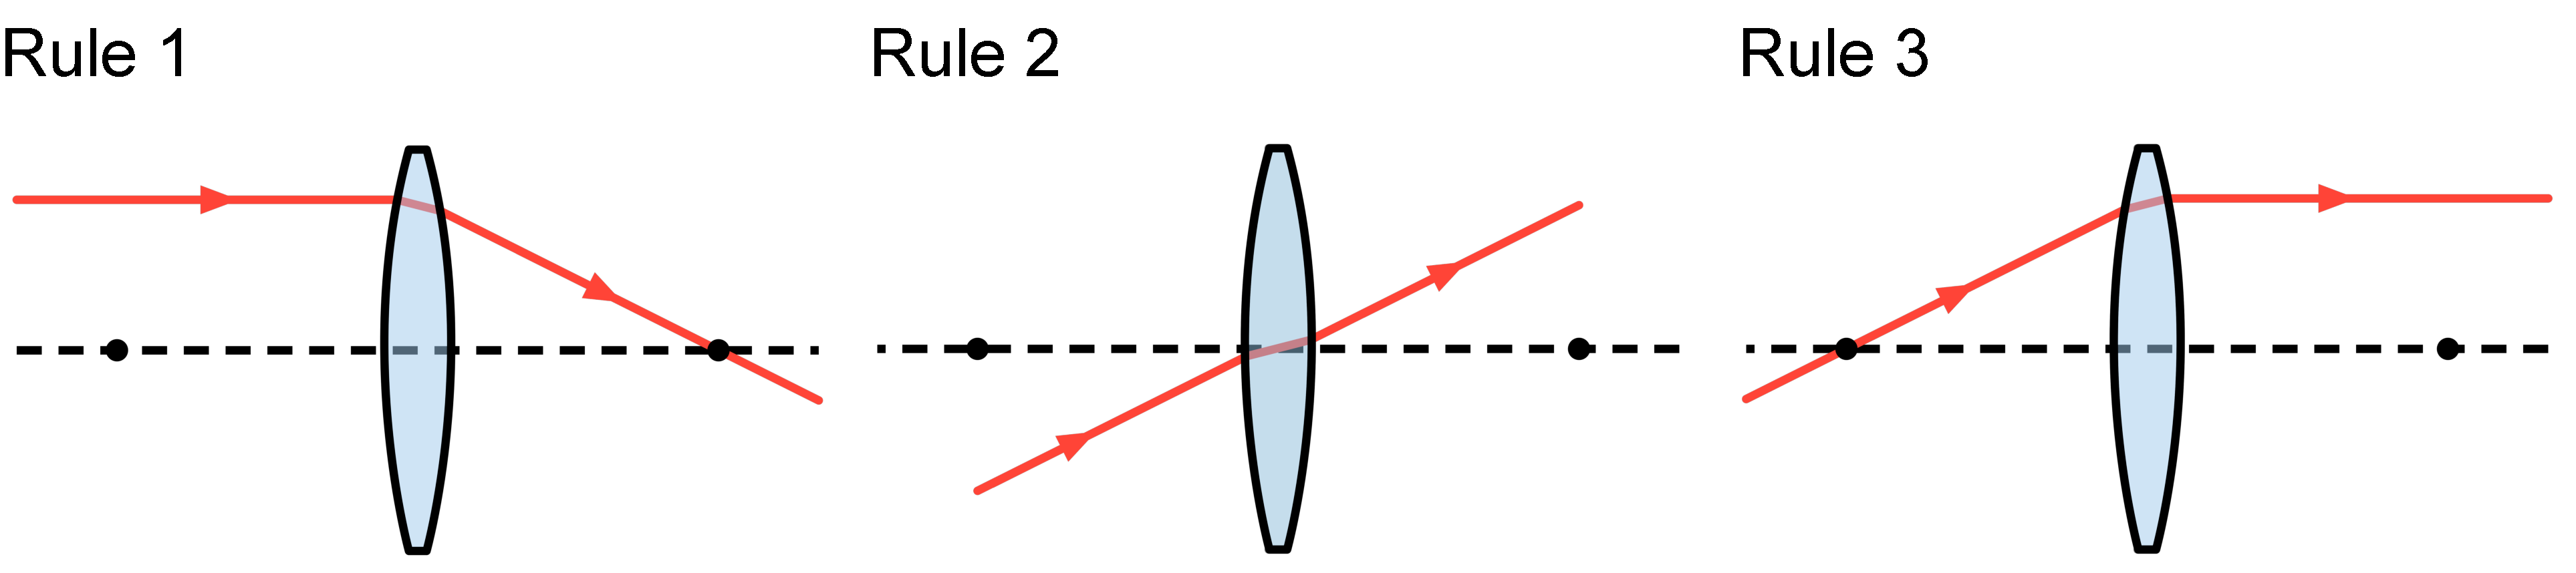
\includegraphics[width=1\linewidth]{Ray Tracing Rules.pdf}
    \caption{The basic rules of ray tracing for a simple lens.}
    \label{fig:ray-tracing}
 \end{figure}

\subsubsection{Thin Lens Equation}

The thin lens equation is a key principle in geometrical optics that describes the relationship between the focal length of a lens, the distance from the object to the lens, and the distance from the resulting image to the lens. It is used to predict how a lens will focus light from an object to form an image. You will use this to measure the focal length of your tube lens.

$\frac{1}{f} = \frac{1}{d_o} + \frac{1}{d_i}$.

Where $f$ is the focal length of the lens, $d_o$ is the object distance and $d_i$ is the image distance.

This equation assumes the lens is thin, meaning its thickness is negligible compared to the object and image distances.

\subsection{Finding the focal length of a lens}

Apply the ray tracing rules to the tip of the a-symmetric arrow in Figure \ref{fig:Single Lens Imaging}. Complete the figure by drawing the image of the object. By measuring the height of the formed imaged, the object distance, $d_o$ and the image distance, $d_i$ calculate the magnification of the image using two different methods. Using the thin lens equation, calculate the focal length of the lens in millimetres.

\begin{figure}
    \centering
    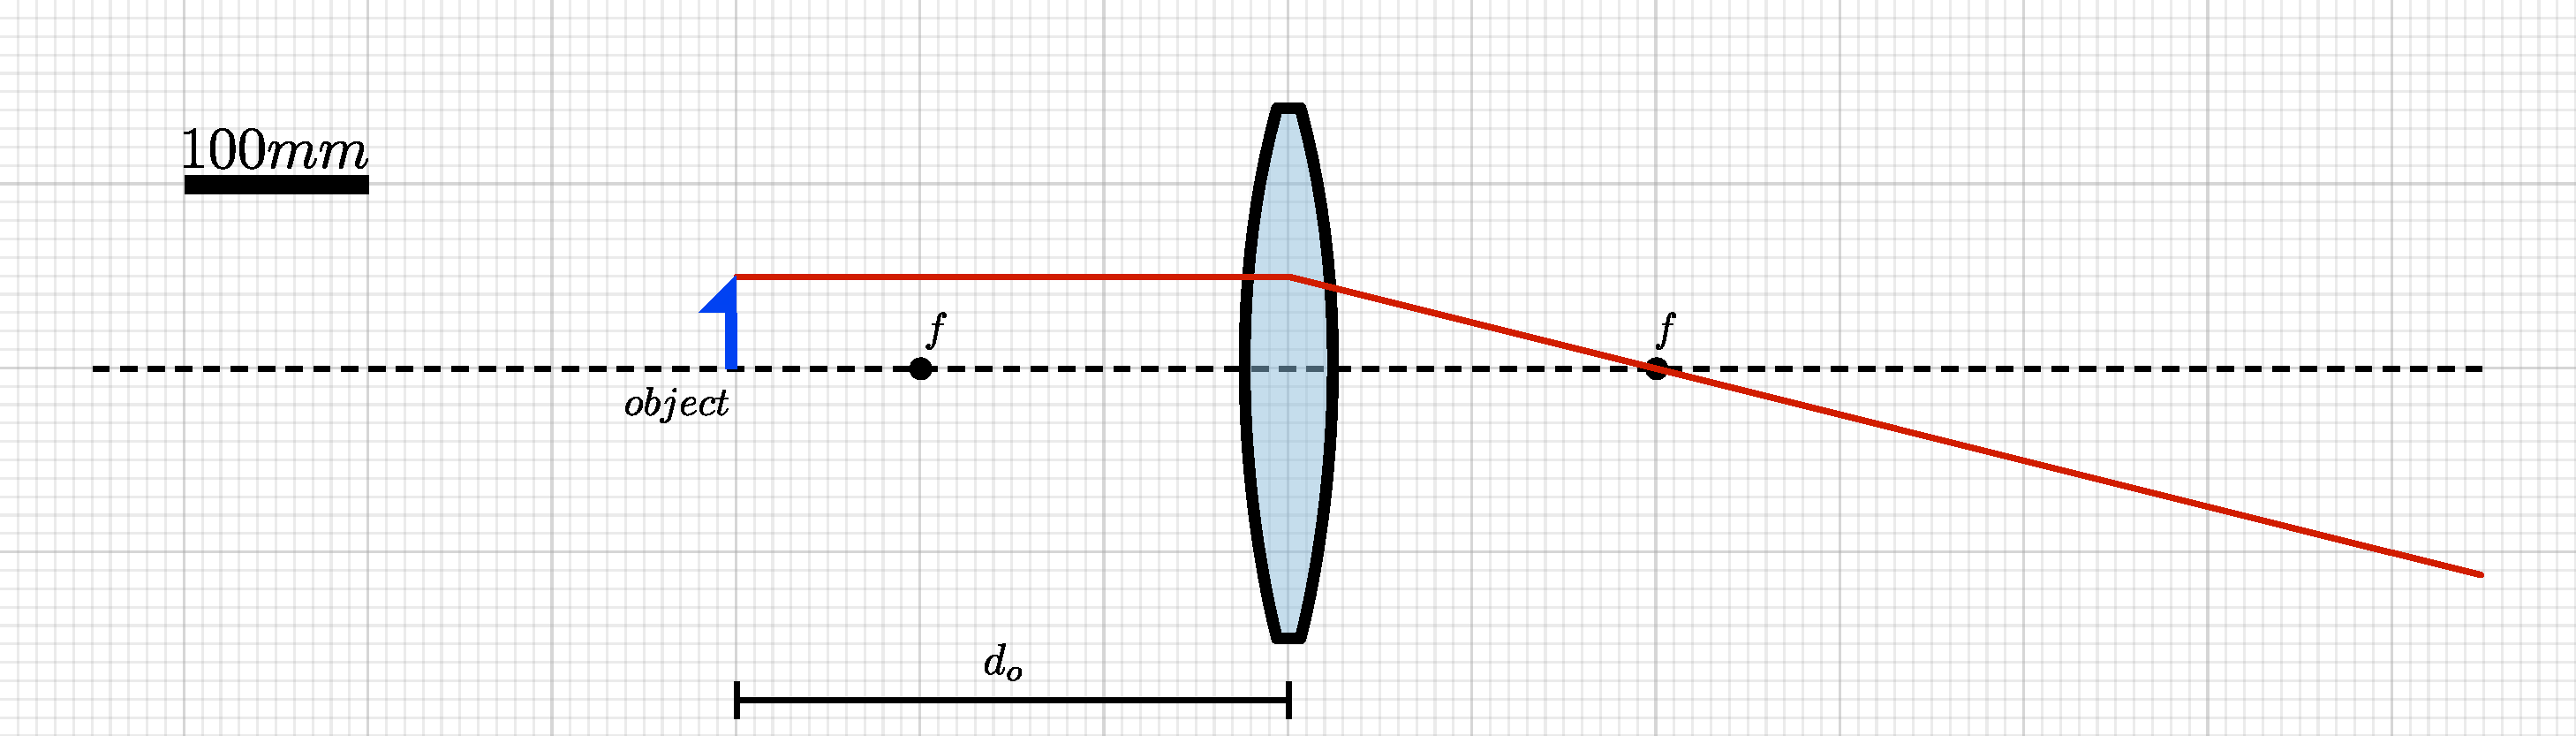
\includegraphics[width=1\linewidth]{Single Lens Imaging.pdf}
    \caption{Forming an image with a single lens.} 
    \label{fig:Single Lens Imaging}
\end{figure}

Focal Length =.        
\subsection{Find the focal length of your tube lens}

First we will find a rough approximation of the focal length of the tube lens. This is done by forming an image of an approximated infinite light source (a ceiling light for example) on the surface of the floor. Measure the distance between the lens and the image to find the approximated focal length, $f_{\approx}$.

$f_{\approx} =$

Why is this method an approximate measure of the focal length?
% A: Since the light incident on the lens is not truly at infinity it is slightly divergent, which results in a image being formed near but not at the focal plane.
Is the measured focal length longer or shorter than the true focal length?
        \vspace{2cm}
% A: Longer. The further away an object plane, the closer the image plane gets to the true focal plane.

\subsubsection{Image Formation with a Single Lens}

Install the alignment target onto the end of four of the rods and install your tube lens at a distance of $2f_{\approx}$ from the target. With the naked eye, find the position where the image of the grid is in focus. What do you notice about the image magnification?
        \vspace{2cm}
% A: The image is inverted and the grid is not magnified.

Move your tube lens 25\% closer to the alignment target (ie a distance of $0.75$ $\times$ $2f_{\approx}$). Observe the image again with the naked eye. What do you notice about the image quality?
        \vspace{2cm}
% The image is magnified this time but the magnification varies across the image, this is an aberration. The system is not telecentric, meaning that the distances from the centre of lens are not the same as at the edges of lens which results in a small variation in magnification across the image. If we observed the image with an equally curved surface we would not see this distortion.

\subsection{Image Formation with Two Lens}

To form an aberration free, magnified image we need to place the object in the focal plane of the lens, however this would result in an image being formed at infinity from the lens (see lens maker equation). So we use two lenses. The first lens, the objective, collects light from the object and the tube lens forms an image at the focal plane of itself. To do this we need a more accurate measurement of the focal length of the tube lens.

\subsubsection{Form same image on camera}

Place alignment grid, tube lens and camera on the alignment rail. Using your approximated focal length of the tube lens, place the lens a distance of $2f_{\approx}$ from the camera sensor. Now place the target grid on the opposite side of the lens and adjust its position until you see a clear image on the camera. Measure the distance between the lens and the target to find the true focal length of the tube lens, $f_t$. Position the tube lens exactly $f_t$ from the camera sensor.

$f_t =$ 

\subsection{Complete scope build}

The set up you are building contains an objective and a tube lens which have different focal lengths. Consider the path of light through both lenses in the diagram below what is the significance of using two lens of different focal length?

\begin{figure}
   \centering
   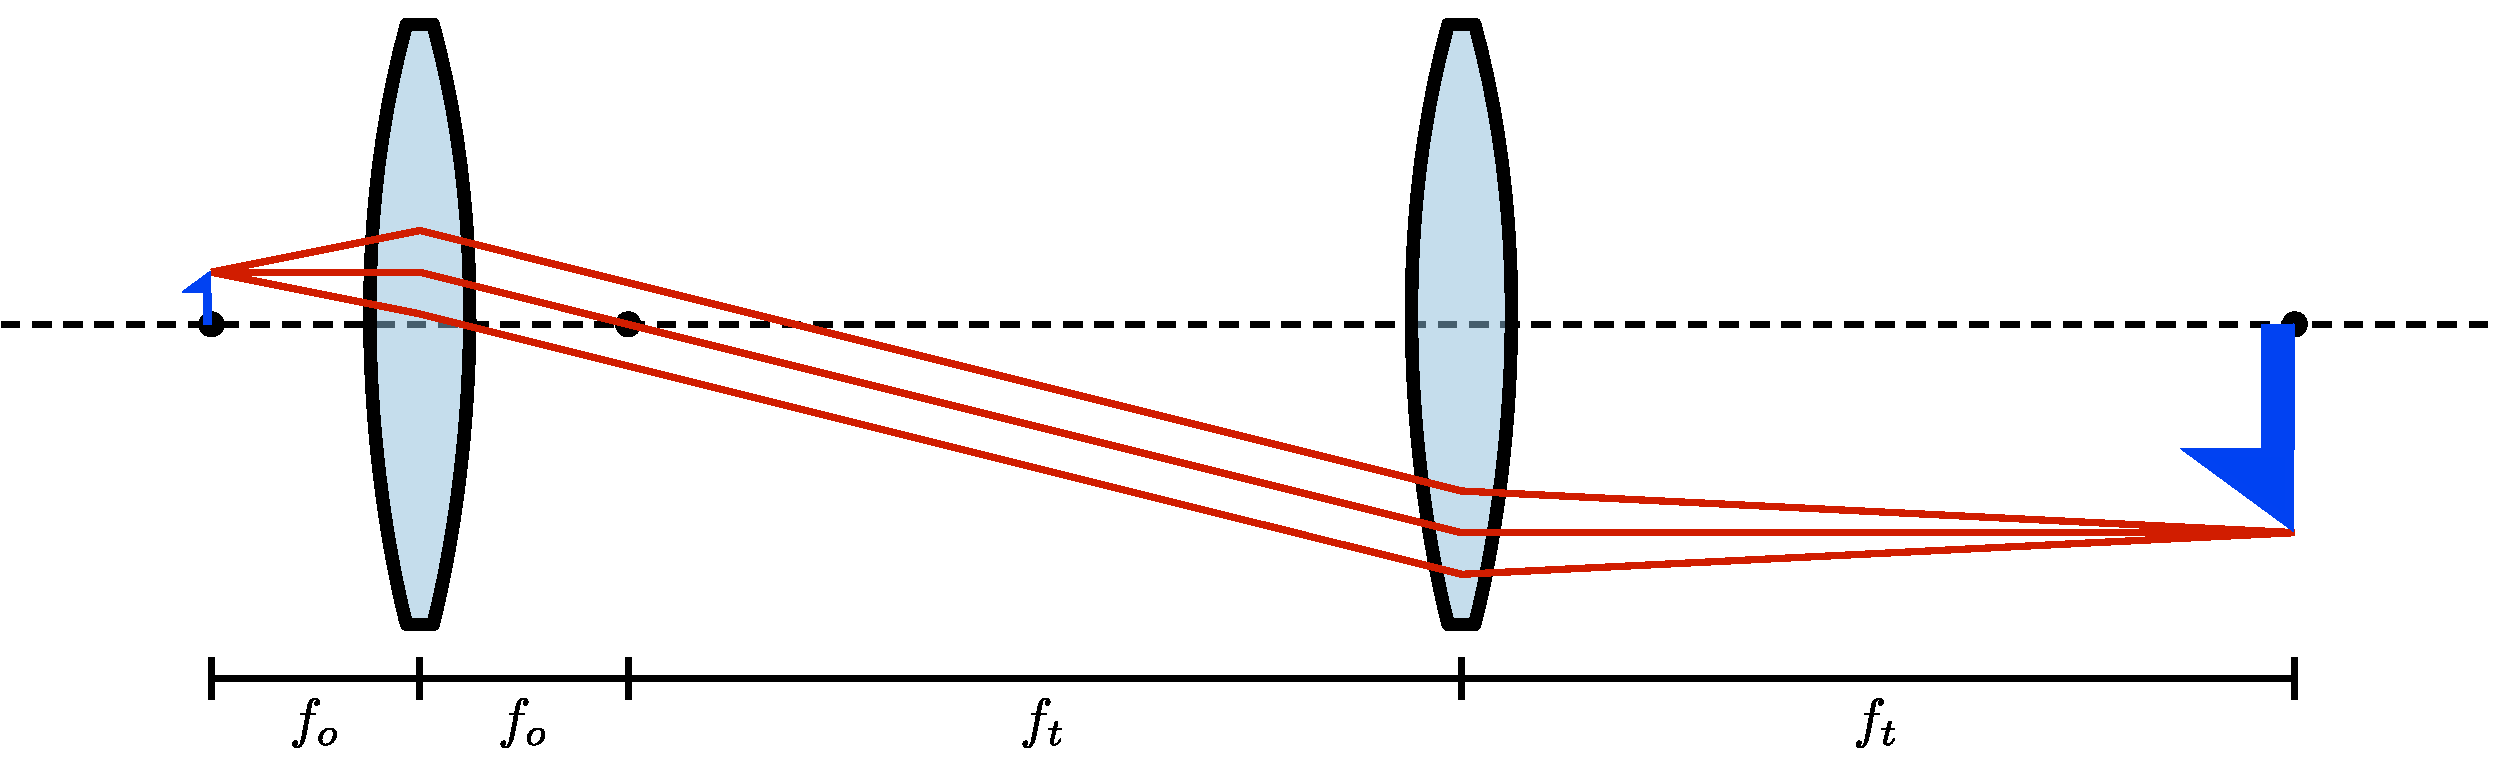
\includegraphics[width=1\linewidth]{Imaging with 4F.pdf}
   \caption{Image formation with an objective and tube lens.}
   \label{fig:4f system}
\end{figure}

Place objective roughly a focal length in front of tube lens. Place the adaptor over the objective and switch on the illumination. Adjust the position of objective until an image of the alignment grid is seen on the camera. TODO: This needs revising to account for the fact that the objective can be placed almost anywhere and still produce an image. Once we have the objectives in the lab we can measure their focal length and instruct students to position the objective at a distance of 2f from the tube lens, using a ruler.

% The overall layout should resemble the diagram below. Illustrate the path of light through your set up and label the components.

% \begin{figure}
%    \centering
%    \includegraphics[width=1\linewidth]{Set Up.pdf}
%    \caption{Enter Caption}
%    \label{Set Up}
% \end{figure}

\subsubsection{Calibrate the camera}

Capture an image of the alignment target and measure the size in pixels (px) of the $10 \mu m$ grid. This gives you the pixels per micrometre calibration so you can convert your images to real world units.

Pixel Size =
\vspace{2cm}
\subsubsection{Measure your microscopes magnification}

Knowing the calibration above and the physical size of each camera pixel ($2$ $\mu m $), calculate the magnification of your microscope.

Magnification =

\vspace{2cm}
Why is your magnification not that stated on your objective?
\vspace{2cm}
% A: An objectives magnification is based on the combination of the objective and a specific tube lens. Your tube lens is not the same as the one intended to be used with this objective.

What is the focal length of your objective?
\vspace{2cm}
% A: f_o = f_t / M

\newpage
\section{Imaging Colloids}

\subsection{Understanding How a Colloid Image is Formed}

Depending on the height the colloids relative to the focal plane of the objective, the image formed will be different. For computational tracking of your colloids the position of the sample is crucial. For optimal tracking we want the image of a colloid to have a bright centre with a dark ring around it. Explain why the dark ring is darker than the background level of your image. Draw a diagram of a colloid with collimated incident rays and show how the rays interact with the curvature of the colloid. Indicate on the drawing where the focal plane of the objective should be for optimum imaging.
\vspace{2cm}

% For broadband, incoherent light the dark ring is mostly due to total internal reflection, where the incident light is at an angle greater than the critical angle for the colloids refractive index. This light is then reflected out of the microscopes optical path and does not reach the camera. The bright centre is due to the light that is incident below the critical angle and is refracted into the colloid. Diffraction only plays a significant role when we illuminate with monochromatic, coherent light.

\subsection{Sizing Colloids}

\begin{itemize}
    \item Add $2$ $\mu l$ of each colloidal suspension (1-11) to a glass slide and leave to dry for $30$ minutes.
    \item Using your microscope, find a concentrated section of colloids where a crystal lattice can be identified.
    \item Draw a line through $3$ or more particles to determine the mean diameter in $\mu m$.
\end{itemize}

    \begin{center}    
        \begin{tabular}{ |c|c|c|c|c|c|c|c|c|c|c|c| } 
            \hline
            & 1 & 2 & 3 & 4 & 5 & 6 & 7 & 8 & 9 & 10 & 11\\
            \hline
            $radius/\mu m$ & \hspace{1cm}  &  \hspace{1cm}   &   \hspace{1cm}  & \hspace{1cm}   &   \hspace{1cm} &   \hspace{1cm} &  \hspace{1cm}  &   \hspace{1cm} &  \hspace{1cm}  &  \hspace{1cm}  &   \hspace{1cm} \\
            \hline
        \end{tabular}
    \end{center}

% This is an approximate of the true size of an object. It needs to be made clear so that students don't progress in their education thinking that sizing small objects is easy.

\subsection{Imaging Parameters}

A key in many-particle tracking is linking up particles positions in a time series of images to form a trajectory for each particle. In order to keep track of each particle, the displacement from image to image needs to be significantly smaller than the mean particle diameter. So we have to capture images at a frame rate that meets this requirement.

To estimate our frame rate we need to know the translational diffusion constant of our particles. This can be calculated from the Stokes-Einstein equation,

\begin{equation}
    D = \frac{k_B T}{6 \pi \eta r},
\end{equation}

where $D$ is the translational diffusion constant, $k_B$ is the Boltzmann constant, $T$ is the temperature, $\eta$ is the viscosity of the solvent and $r$ is the radius of the particle.

Given that $\langle x^2 \rangle = 2 D \tau$ calculate the time, $\tau$ it takes for a particle to move a distance equal to its diameter, $d$.

\begin{center}    
    \begin{tabular}{ |c|c|c|c|c|c|c|c|c|c|c|c| } 
        \hline
        & 1 & 2 & 3 & 4 & 5 & 6 & 7 & 8 & 9 & 10 & 11\\
        \hline
        $\tau/s$ & \hspace{1cm}  &  \hspace{1cm}   &   \hspace{1cm}  & \hspace{1cm}   &   \hspace{1cm} &   \hspace{1cm} &  \hspace{1cm}  &   \hspace{1cm} &  \hspace{1cm}  &  \hspace{1cm}  &   \hspace{1cm} \\
        \hline
    \end{tabular}
\end{center}

What is the lowest frame rate you can use such that the colloid will be trackable from frame to frame?
\vspace{2cm}

Select one batch to continue with. What was the reasoning behind this choice?
\vspace{2cm}

Create a sample using the instructions in the sample preparation area. Ensure your colloids are diluted such that you end up with a monolayer of colloids when imaging them. Start with a dilution of $1$ $mL$ of water to $1$ $\mu L$ of colloid solution. Let your sample sediment for $\approx$ $5$ minutes on the microscope then check to see if you have a monolayer.

Once you have a monolayer, capture a series of images at the frame rate you estimated earlier.

TODO: How many images?

\newpage
\section{Tracking and Analysis}

In this section you will use Matlab to analyse your microscopy images. 

The code can be found at: \href{github.com/Dullens-Lab/Matlab-Particle-Tracking}{github.com/Dullens-Lab/Matlab-Particle-Tracking}

Particle tracking can be divided into 3 main sections;

\begin{itemize}
    \item Image Processing
    \item Particle Location
    \item Particle Tracking
\end{itemize}

In words first the raw images are cleaned up, then the particle coordinates in each frame are found and finally these coordinates are linked up to form trajectories connected to an individual particle.

First you will work through a tutorial on image processing and particle location and then you will build these routines into a loop to find particles your own data. Finally the particle coordinates will be tracked.

\begin{itemize}
    \item In Matlab open the file \lstinline{Tutorial.m}.
    \item Use run section to load the example image into the workspace.
    \item Use the command \lstinline{imagesc()} or \lstinline{imshow()} to display the image.
\end{itemize}

\subsection{Image Processing}

Particle location relies on having good images where the only features are the colloids themselves. The image filtering step filters high and low frequency noise and applies a fixed background subtraction such that the background equals a pixel value of $0$. Open the function file \lstinline{bpass.m} and read through the code.

\begin{itemize}
    \item What is the background value of the raw image?
    \item Open the function file \lstinline{bpass.m}.
    \item Define the inputs to the function.
    \vspace{1cm}

    \item Run the function with the following inputs: \lstinline{bpass(image, true, true, 3, false)}.
    \item Change the value for the background until all the background is removed.
    \item Save the filtered image.
    \item Change the input for ns and nl to integers and try to replicate the same filtered image. Record your final values below.
        \vspace{1cm}
         \item How does your value for ns and nl relate to the size of the particle?
        \vspace{1cm}   
\end{itemize}



\subsection{Particle Location}

Once the image is processed the particle locations can be found. This takes places via a two step process where the rough location is found to the nearest pixel and then the fit is refined with subpixel accuracy. 

\begin{itemize}
    \item Open the function pkfnd.
    \item Define the inputs.
        \vspace{1cm}
    \item Define the outputs.
        \vspace{1cm}
    \item On what basis is the particle centre found?
        \vspace{1cm}
      \item Run this section with the following inputs: $pkfnd(filtered,10,3)$
        \vspace{1cm}   
    \item Find the peaks in the raw and the filtered image, how would tracking unprocessed images affect results?
        \vspace{1cm}
\end{itemize}

 Once the rough peaks are found the positions are refined by a subpixel fitting routine

\begin{itemize}
    \item Open the function cntrd
    \item Describe in words how the fitting is carried out
        \vspace{1cm}
    \item Define the output
        \vspace{1cm}
     \item Run this section with the following inputs: $cntrd(filtered,estpks,5,true,1)$
        \vspace{1cm}   
\end{itemize}

%Pixel Biasing

Create a figure either in Matlab or Powerpoint of the raw, filtered, filtered with rough positions and filtered with refined positions.

\subsection{Create Tracking Loop}
A convenient way to store information in Matlab uses structures where each field within a structure contains an array e.g. if COORD is a structure with one field, cntrds, the positions for frame t can be stored in COORD(t).cntrds.
Rewrite the tracking procedure as a loop over all frames where the final coords are found in the structure COORD.
Note before the coordinates are stored add a fourth column containing the timepoint. Your loop should not involve showing/plotting anything.

\subsection{Particle Tracking}

Once we have the particle locations in each frame we must link them up to form trajectories. 

\begin{itemize}
    \item Open the track function.
    \item Define the inputs.
    \vspace{1cm}
    \item Define the outputs.
        \vspace{1cm}
    \item Track the particles using the diameter as the maximum displacement
\end{itemize}

\subsection{Analyse Your Own Data}
Run you tracking loop over your own data. (Not you will have to optimise the parameters for each step, you can use the tutorial script for this).


\subsection{Mean Square Displacement}

What shape do you expect the MSD to be?
    \vspace{1cm}
What function should fit the line?
    \vspace{1cm}

\subsubsection{Calculate the MSD}

\begin{itemize}
    \item Import the MSD function into the correct workspace
    \item Run this function (input = (x y z t ID)
    \item Output of this function is the ensemble averaged MSD, describe in a sentence how this averaging is being carried out.
    \item Plot the MSD versus time (in seconds)
\end{itemize}

\subsubsection{Fitting the MSD}

\begin{itemize}
    \item Using the Matlab function $fit$ fit the MSD versus t(s) with the correct function
    \item From this value determine $D_T$. What are the units?
        \vspace{1cm}
    \item What is the value of $D_T$ after fitting over 10 points vs 1000 points? Which is likely to be more accurate
        \vspace{1cm}
    \item From your $D_T$ determine Avagadro's Number.
        \vspace{1cm}
\end{itemize}

\newpage
\section{Optical Trapping}

In this section you will utilise the technique of optical trapping to again determine Avagadro's number. Optical trapping is a technique used across many field of science that uses a laser light source to 'trap' a probe which allows direct manipulation and measurements of forces within a sample.

Optical trapping relies on a refractive index mismatch between particle and solvent. 
What type of light source is a laser?
\vspace{2cm} 

Consider the Fig. \ref{fig:trap} which shows a colloidal particle trapped within a laser beam and a particle displaced from the centre of the beam.
Consider the first senario:
\begin{itemize}
	\item What two things happens to the incident ray when it hits the particle?
	\vspace{2cm}
	\item Label the two resultant forces on the particle from both effects?
	\vspace{2cm}
	\item Therefore explain why a refractive index mismatch between particle and solvent is important.
	\vspace{2cm}
\end{itemize}

Consider the second senario:
\begin{itemize}
	\item What two things happens to the incident ray when it hits the particle?
	\vspace{2cm}
	\item Label the two resultant forces on the particle from both effects?
	\vspace{2cm}
	\item For the particle to be restored to the trap which force must be greater?
\end{itemize}

\begin{figure}
    \centering
    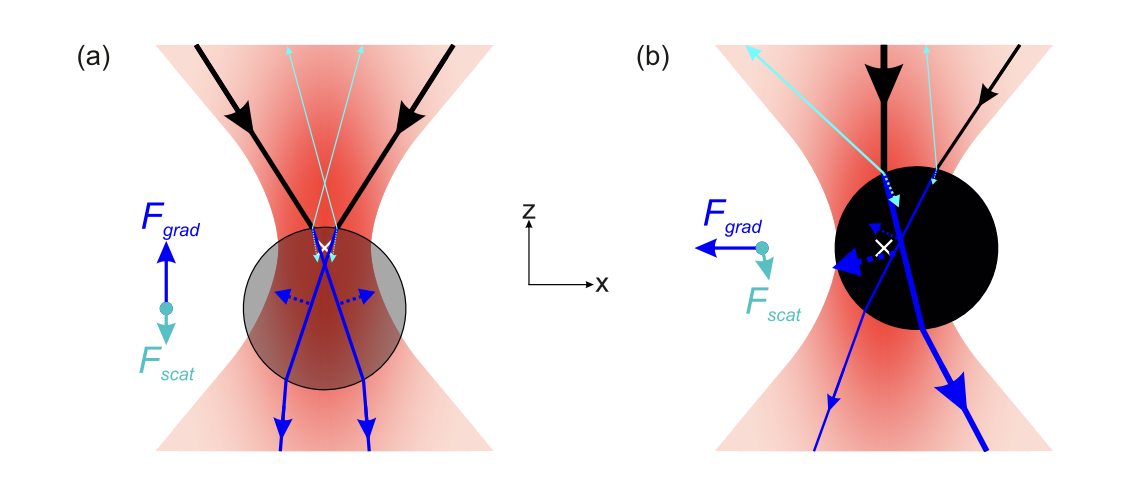
\includegraphics[width=1\linewidth]{Trapping.png}
    \caption{Forces in Optical Trapping.}
    \label{fig:trap}
\end{figure}

Sample should be prepped in an identical way to the previous microscopy experiments.

\subsection{Safety}
In this section you will carry out this experiment in the laser lab of PCSM. This set up includes a Class IV laser, this is the most dangerous type of laser which can cause serious eye damage. You must adhere to the following safety procedures:

\begin{itemize}
    \item Laser Safety glasses must be worn at all times in the laser lab
    \item Failure to listen to instructions from supervisors will result in a penalty to your grade.
\end{itemize}

\subsection{Analysis}
\begin{itemize}
	\item Using the particle location and tracking loop you developed previously calculate the MSD for the trapped particle. 
	\item How is is different to the 'free' particle?
	\vspace{2cm}
\end{itemize}

 A particle on in a trap can be compared to a particle on a spring. We can determine the stiffness of the trap using Hooke's Law.
 \begin{itemize}
	\item What is Hooke's law for the potential energy of a spring?
	\vspace{2cm}
\end{itemize}
	
$U(r)$ can be approximated as the $-ln(P(r))$, where r is the displacement of the particle. 
 \begin{itemize}
	\item Copy the code for MSD into a new file and adapt it to plot ln(P(r).
	\item Fit this with the relation given by Hooke's Law to determine the trap stiffness.
	\vspace{2cm}
\end{itemize}

The trap stiffness can be related to Boltzmann constant by the equation;

$ \langle x^2 \rangle = k_b \frac{T}{\alpha} $

where $\alpha$ is the trap stiffness. 

 \begin{itemize}
\item Use this relation to determine Boltzmann constant and in turn Avagadro's number.
          \vspace{2cm}
\item Which method was more accurate and why?
	\vspace{2cm}
\end{itemize}

\newpage

\section{Report}
You may use either Word or LateX to complete your report. It should follow the following layout:


\subsection{Introduction}
Describe the work of Perin (Prep work) and state the aim of this Practical.

\subsection{Experimental Details and Theory}
\subsubsection{Colloidal Model System}
 \begin{itemize}
	\item Define a Colloid.
	\item Define Brownian Motion, MSD and how to calculate $D_T$.
	\item Describe why colloids can be used as 'big atoms'.	
\end{itemize}

\subsubsection{Synthesis}
 \begin{itemize}
	\item Explain mechanism of synthesis of colloidal particles from TPM.
	\item Outline Ppocedure followed.
	\item Include images and sizes for all batches.
	\item Include what batch was chosen for further experiments and why.	
\end{itemize}

\subsubsection{Micrscopy}
 \begin{itemize}
	\item Include the diagram provided and draw the path of light through the set up.
	\item Define ach component.
	\item Define the focal length and give the determined value.
	\item Give the determined pixel size of the camera and magnification of the microscope.
	\item Give the final image parameters and explain the values.
\end{itemize}

\subsubsection{Tracking}
 \begin{itemize}
	\item Include the raw tutorial image as well as the same image after each step.
	\item Describe the process of image processing, particle location and tracking.
\end{itemize}

\subsubsection{Optical Trapping}
 \begin{itemize}
	\item Include the diagram provided with the completed ray diagram.
	\item Describe the forces acting on the particle.
	\item Describe how the magnitude of the forces dictate if the particle remains in the trap.
\end{itemize}

\subsection{Results}

\subsubsection{Determination of Avagadro's Number from MSD}
 \begin{itemize}
	\item Show graph of MSD against time.
	\item Give value of Dt and NA.
	\item Explain any sources of discrepancy in your answer.
	\item How is this method an improvement on Perrin's work.
\end{itemize}

\subsubsection{Determination of Avagadro's Number from k}
 \begin{itemize}
	\item Show graph of MSD against time.
	\item Show graph of U vs r.
	\item Give value of k and NA.
	\item Explain any sources of discrepancy between your two values.
\end{itemize}

\end{document}








